\documentclass{LabReport}


% import packages
\usetikzlibrary{shapes,arrows}


% cover information
\CourseTitle{EIE3810 Microprocessor System Desgin \par Laboratory}
\ReportTitle{Laboratory Report \#X}
\StudentName{XXXXXXXXX}
\StudentID{XXXXXXXXX}
\ReportDate{XXXXXXXXXX}
\Institution{The Chinese University of Hong Kong, Shenzhen}


% start the document
\begin{document}

% make cover page
\makeCover

% set basic char layout
\setstretch{1.5} % line spacing
\setlength{\parskip}{0.2em} % distance between paragraphs
\fontsize{12}{1em} % font size
\setmainfont{Times New Roman} %  font face
% \setlength{\spaceskip}{0.35em} % distance between char
\justifying

% start counting page
\pagenumbering{arabic}

% introduction
\setlength{\parindent}{0em}
In Lab \#X, we learned about how to include figures, codes, and flowchart in Latex. More commands are all in .cls file, including how to set the information and how to mark a 'TO BE WRITTEN'. You can go to this file for details.
\setlength{\parindent}{1.5em}

\setlist[itemize]{topsep=0pt,partopsep=0pt,parsep=0pt,itemsep=0pt}
\begin{itemize}[leftmargin=1em]
    \item [$\bullet$] Experiment A: Include figures in Latex.    
    \item [$\bullet$] Experiment B: Include codes in Latex.
    \item [$\bullet$] Experiment C: Include flowchart in Latex.
\end{itemize}


% other contents
\section{Experiment A}

\subsection{Design}
This experiment is to include figures in Latex.

\subsection{Result}
The result is shown below.

\begin{figure}[H]
    \centering
    
\includegraphics[width=12cm]{figures/boy.jpeg}
    \caption*{\textbf{Figure 1.2.1} ~ The result of including picture boy.jpeg}
\end{figure}

\subsection{Quetion}

\setlength{\parindent}{0em}

\textbf{Question1:} Why we need the command to set parindent to ask a question?

\textbf{Answer:} Because we want to set the paragraph indent to 0, which means the first line of the paragraph will not be indented.

\setlength{\parindent}{1.5em}

\section{Experiment B}

\subsection{Design}
This experiment is to include codes in Latex.

\subsection{Result}

\lstinputlisting[language=c, caption=\textbf{Code 2.1.1} ~ The implementation of main.c]{codes/helloworld.cpp}

\section{Experiment C}

\subsection{Design}
This experiment is to include a flowchart in Latex.

I thinks write a flowchart in Latex is a little bit difficult. Perhaps, just use a picture instead? I think other tools to draw the flowchart is much easier.

\subsection{Result}

\begin{center}
    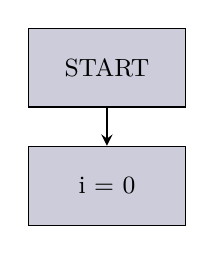
\begin{tikzpicture}[node distance=2cm, auto]
        \setmainfont{Hack}
        \fontsize{9}{1em}

        % define shape
        \tikzstyle{process} = [rectangle, minimum width=2cm, minimum height=1cm, text centered, aspect=2,draw=black, fill=blue!30!black!20!]
        \tikzstyle{test}=[diamond,aspect=2,draw=black, fill=yellow!30!black!20!]
        \tikzstyle{round}=[rounded rectangle,aspect=2,draw=black,fill=green!30!black!20!]
        \tikzstyle{point}=[coordinate]

        % define content
        \node (START) [process] {START};
        \node (init) [process, below of=START, node distance=1.5cm] {i = 0};
        % connect flow chart
        %\draw[->] (n0.south) -- (n1); arrow
        %\draw[-] (n0.south) -- (n1); no arrow
        %\draw[<->] (n0.south) -- (n1.north);   double arrow
        %\draw[<-,dashed] (n1.south) -- (n2.north); dash arrow
        %\draw[<-] (n0.south) to node{Yes} (n1.north);  word right
        %\draw[->] (n1.north) to node{Yes} (n0.south);  word left
        %\draw[->] (n1.north) to[out=60,in=300] node{Yes} (n0.south);  curve
        %\draw[->,draw=red](n2)--(n1);  line with color
        \draw[thick, ->, >=stealth] (START) -- (init);
        
    \end{tikzpicture}
\end{center}

\section{Conclusion}

In Lab \#X, we learned about how to include figures, codes, and flowchart in Latex.

This template will be updated in the furture. If you have any questions about this report template, please feel free to contact me via email {\textcolor{blue}{shinoxiaoyu@outlook.com}}. Thank you for your reading.

\end{document}